\section{Introduction}
\label{sec:introduction}

\IEEEPARstart{I}{ndustrial} control commands increasingly cross organizational and network boundaries before they reach a physical process. Maintenance services, supervisory applications, and autonomous software principals may receive authority to inspect or actuate assets in another security zone~\cite{iec62443}. Network segmentation constrains where communication can flow, but delegated actuation also depends on the target asset, operation, physical parameter, time, operating mode, and preceding events. A runtime authorization object must preserve these restrictions as authority moves between principals. More importantly, an industrial operator needs to know whether narrowing that object also narrows the physical behavior the delegate can induce.

Capability systems offer a natural basis for delegated least privilege. Cyber-physical capability architectures combine local architectural protection with cryptographic tokens~\cite{dodson2021,dodson2020}, and recent agent-facing systems add signed physical constraints, attenuation, revocation, approvals, and audit~\cite{sint2026,ranathunga2026,bamil2026}. Their digital ordering does not, by itself, order plant behavior. A child may submit different requests from its parent, and an enforcement layer may replace, delay, or suppress those requests. Syntactic scope inclusion must therefore be connected to the set of physical inputs actually emitted at runtime.

Physics-aware access control and runtime enforcement address the downstream problem from complementary directions. Model-informed policies can reject actions whose predicted consequences violate a physical condition~\cite{etigowni2016,rafy2026}. Edit-automata and industrial I/O enforcers can suppress or correct compromised-controller events, with established soundness, progress, and scalability properties~\cite{ligatti2005,pearce2020,lanotte2023,baird2024}. Separately, IEC~62443-3-2 structures industrial risk assessment around zones and conduits~\cite{iec62443}. These lines do not specify a common refinement relation from zone/conduit-derived delegation syntax, through a command-editing enforcement point, to the physical traces admitted by the plant.

This paper introduces \zonecap{}, which makes that missing interface explicit. A source-table compiler converts directed zone/conduit grants and declared physical caveats into capabilities, while a field-wise validator restricts every delegated child. At runtime, five authorization effects map requests to checked physical emissions, registered holds, or no actuation event. The central insight is a three-step refinement: positive conjunctive attenuation establishes authorization inclusion; sound and parent-realizable effects establish request-abstracted emission inclusion; and a common plant relation lifts emission inclusion to finite-horizon trace and reachable-set inclusion. Fig.~\ref{fig:overview} summarizes the path.

\begin{figure*}[t]
\centering
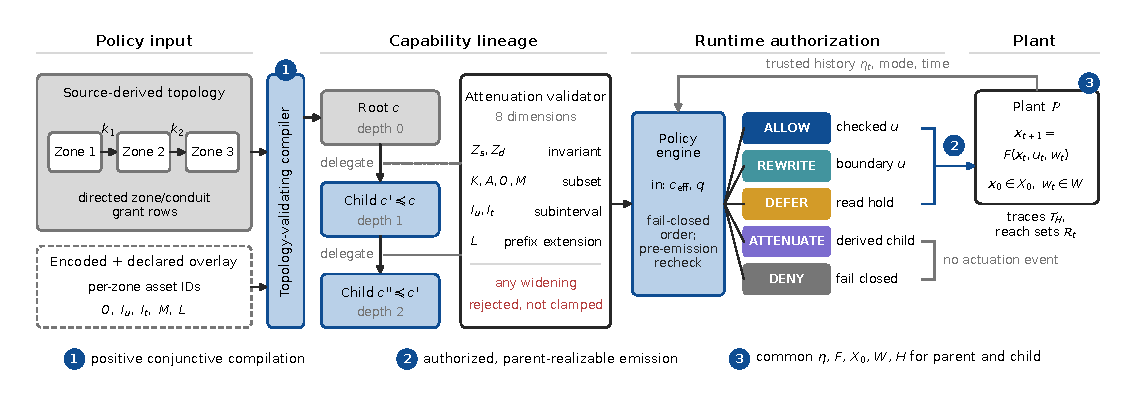
\includegraphics[width=\textwidth]{figures/generated/fig01_zonecap_overview}
\caption{ZoneCap compilation, delegation, enforcement, and physical-refinement path. The grey block is the source-derived zone/conduit topology; the dashed block holds per-zone asset identifiers and the declared evaluation overlay, which the sources do not supply. The validator checks eight authority dimensions without querying plant reachability. \texttt{DENY} and \texttt{ATTENUATE} emit no actuation event; the figure depicts actuation-event semantics, not fixed-tick PLC execution. Numbered badges mark the interfaces at which Section~\ref{sec:theorem} imposes obligations: (1)~positive conjunctive compilation, (2)~authorized and parent-realizable emission, and (3)~a common history projection, plant relation, uncertainty set, and horizon for parent and child.}
\label{fig:overview}
\end{figure*}


The paper makes the following contributions:
\begin{itemize}
    \item It establishes a conditional refinement theorem from field-wise capability attenuation to physical trace and reachable-set inclusion. Six explicit obligations separate the result from same-request behavior, controller synthesis, and model-mismatch robustness.
    \item It develops a zone/conduit-table compiler and validates it on frozen CPwE/CIP Security and ENISA landside-signalling inputs augmented by a declared source-independent overlay. Complete-corpus, mutation, provenance, path, and delegation checks test the concrete realization.
    \item It defines an actuation-event semantics for \texttt{ALLOW}, \texttt{DENY}, \texttt{ATTENUATE}, \texttt{REWRITE}, and \texttt{DEFER}, and evaluates refinement, composition, effect coverage, and deny-only service loss in the registered bounded model.
\end{itemize}
The evaluation also reports a negative result: fair delayed revocation delivery admits issuance-relative stale execution even when resolver-local post-delivery invariants remain intact. This boundary shows that physical refinement and lifecycle safety require explicit operational contracts rather than an unqualified claim of safe attenuation.
